%%%%%%%%%%%%%%%%%%%%%%%%%%%%%%%%%%%%%%%%%%%%%%%%%%%%%%%%%%%%%%%%%%%%%%%%%%%%%%%%
%2345678901234567890123456789012345678901234567890123456789012345678901234567890
%        1         2         3         4         5         6         7         8

\documentclass[letterpaper, 10 pt, conference]{ieeeconf}  % Comment this line out if you need a4paper
%\IEEEoverridecommandlockouts                              % This command is only needed if 
                                                          % you want to use the \thanks command
%\overrideIEEEmargins                                      % Needed to meet printer requirements.
% See the \addtolength command later in the file to balance the column lengths
% on the last page of the document
%\documentclass{article}

% The following packages can be found on http:\\www.ctan.org
\usepackage[pdftex]{graphicx} % for pdf, bitmapped graphics files
\graphicspath{{Figures/}}
\pdfminorversion=7
%\usepackage{epsfig} % for postscript graphics files
%\usepackage{mathptmx} % assumes new font selection scheme installed
%\usepackage{times} % assumes new font selection scheme installed
\usepackage{amsmath} % assumes amsmath package installed
%\usepackage{amssymb}  % assumes amsmath package installed
%\usepackage[numbers,sort&compress]{natbib}
%\usepackage{IEEEtran}


\usepackage{spconf}
\usepackage{glossaries}
\usepackage[breaklinks,hidelinks]{hyperref}

\title{Impact of susceptibility distortions in connectivity analysis}

\name{%
\shortstack{Oscar Esteban$^{1,2}$, %
Alessandro Daducci$^{2}$, %
Emmanuel Caruyer$^{3}$, %
Kieran O'Brien$^{4}$,\\%
Mar\'ia Jes\'us Ledesma-Carbayo$^{1}$, %
Meritxell Bach-Cuadra$^{2}$, %
and Andr\'es Santos$^{1}$}%
}

\address{%
$^{1}$Biomedical Image Technologies (BIT), ETSI Telecom.,
U. Polit\'ecnica de Madrid and CIBER-BBN, Spain. \\
$^{2}$ Signal Processing Laboratory (LTS5), \'Ecole Polytechnique
F\'ed\'erale de Lausanne (EPFL), Lausanne, Switzerland. \\
$^{3}$ Section of Biomedical Image Analysis, Dept. of Radiology,
University of Pennsylvania, Philadelphia, PA, USA. \\
$^{4}$  Department of Radiology, University of Geneva, Geneva, Switzerland.
}


%\name{Oscar Esteban$^{1,2}$, Alessandro Daducci$^{2}$, Emmanuel Caruyer$^{3}$, Kieran O'Brien,\\
%Mar\'ia Jes\'us Ledesma-Carbayo, Meritxell Bach-Cuadra, and Andr\'es Santos% <-this % stops a space

%\author{%
%Oscar Esteban$^{1,2}$,%
%Alessandro Daducci$^{2}$,%
%Emmanuel Caruyer$^{3}$,%
%Kieran O'Brien$^{4}$, \\%
%Mar\'ia Jes\'us Ledesma-Carbayo$^{1}$,%
%Meritxell Bach-Cuadra$^{2}$,%
%and Andr\'es Santos$^{1}$
%}

% List of acronyms used in the text
\newacronym{mr}{MR}{magnetic resonance}
\newacronym{mri}{MRI}{magnetic resonance imaging}
\newacronym{dmri}{dMRI}{diffusion MRI}
\newacronym{fmri}{fMRI}{functional MRI}
\newacronym{dw}{DW}{diffusion weighted}
\newacronym{dti}{DTI}{diffusion tensor imaging}
\newacronym{t1}{T1}{T1-weighted}
\newacronym{t2}{T2}{T2-weighted}
\newacronym{csf}{CSF}{cerebrospinal fluid}
\newacronym{wm}{WM}{white matter}
\newacronym{gm}{GM}{grey matter}
\newacronym{epi}{EPI}{echo-planar imaging}
\newacronym{gre}{GRE}{gradient echo sequence}
\newacronym{fa}{FA}{fractional anisotropy}
\newacronym{md}{MD}{mean diffusivity}
\newacronym{adc}{ADC}{apparent diffusion coefficient}
\newacronym{acwe}{ACWE}{active contours without edges}
\newacronym{adf}{ADF}{active deformation field}
\newacronym{map}{MAP}{maximum a posteriori}
\newacronym{snr}{SNR}{signal-to-noise ratio}
\newacronym{pve}{PVE}{partial volume effect}
\newacronym{roi}{ROI}{region of interest}
\newacronym{mrf}{MRF}{Markov Random Field}
\newacronym{psf}{PSF}{point-spread function}
\newacronym{se}{SE}{Surface error}
\newacronym{wi}{WI}{Warping index}
\newacronym{nof}{NoF}{number of fibers}
\newacronym{hardi}{HARDI}{high angular resolution diffusion imaging}
\newacronym{tpm}{TPM}{tissue probability map}
\newacronym{fft}{FFT}{fast fourier transform}
\newacronym{vsm}{VSM}{voxel shift map}

\newacronym{fmb}{FMB}{fieldmap-based}
\newacronym{reb}{REB}{reversed encoding-based}
\newacronym{t2b}{T2B}{T2 registration-based}

\newacronym{frr}{FRR}{fiber recovery ratio}
\newacronym{fji}{fJI}{fuzzy Jaccard's Index}
\newacronym{dwi}{DWI}{diffusion weighted image}

\makeglossaries

%\acrodef{mr}[MR]{magnetic resonance}
%\acrodef{mri}[MRI]{magnetic resonance imaging}
%\acrodef{dwi}[DWI]{diffusion weighted imaging}
%\acrodef{dw}[DW]{diffusion weighted}
%\acrodef{dti}[DTI]{diffusion tensor imaging}
%\acrodef{t1}[T1]{T1-weighted}
%\acrodef{t2}[T2]{T2-weighted}
%\acrodef{csf}[CSF]{cerebrospinal fluid}
%\acrodef{wm}[WM]{white matter}
%\acrodef{gm}[GM]{grey matter}
%\acrodef{epi}[EPI]{echo-planar imaging}
%\acrodef{fa}[FA]{fractional anisotropy}
%\acrodef{md}[MD]{mean diffusivity}
%\acrodef{acwe}[ACWE]{active contours without edges}
%\acrodef{map}[MAP]{maximum a posteriori}
%\acrodef{snr}[SNR]{signal-to-noise ratio}
%\acrodef{pve}[PVE]{partial volume effect}
%\acrodef{roi}[ROI]{region of interest}



\begin{document}



\maketitle
\thispagestyle{empty}
\pagestyle{empty}


\begin{abstract}
Connectivity analysis on diffusion MRI data of the whole-brain
suffers from distortions caused by the standard 
echo-planar imaging acquisition strategies. %
%These artifacts are present at interfaces between tissues,
%due to the inhomogeneity of the field derived from the 
% discontinuity of magnetic susceptibility.
These images show characteristic geometrical deformations
and signal destruction that are a significant pitfall
limiting the success of tractography algorithms.

Several retrospective correction techniques are readily
available. In this work, we use a digital phantom designed
for the evaluation of connectivity pipelines. We subject
the phantom to a ``theoretically correct'' and plausible
deformation that resembles the artifact under investigation.
We correct data back, with three standard methodologies
(namely fieldmap-based, reversed encoding-based, and
registration-based). Finally, we rank the methods based
on their geometrical accuracy, the dropout compensation,
and their impact on the resulting tractography.
\end{abstract}%
\begin{keywords}
susceptibility artifacts, diffusion MRI, tractography, connectivity.
\end{keywords}
\section{INTRODUCTION}
\label{sec:intro}
In-vivo whole-brain connectivity analysis has been a research topic of high
  interest for the last 5 yr.
\Gls*{dmri} can be used to probe the orientation of fiber bundles within the
  brain, and it is generally acquired with an \gls*{epi} sequence.
After signal reconstruction, tractography algorithms draw a map of the sampled
  structures.
These maps can represent the actual trajectories of fiber bundles
  (deterministic tractography) or pixel-wise probability of connection
  to a certain origin (probabilistic tractography).
Finally, the information about these connections is collected into a network
  matrix that is subjected to the ``connectome analysis''.

Among all the difficulties that such a complex workflow raises \cite{jones_twenty-five_2010},
  we will address here the susceptibility-derived artifacts,
  for which \Gls*{epi} schemes are especially sensitive.
Magnetic susceptibility disturbs the magnetic field close to tissue interfaces.
This inhomogeneity of the field translates into a highly distorted anatomy
  and a significant signal destruction in certain regions of the brain 
  (e.g. the orbitofrontal lobe, for the proximity of the air surrounding sinuses).
This artifact has been well described, generally within the context of functional MRI,
  which also uses \gls*{epi}.

Various approaches have been proposed to correct for this distortion.
\Gls*{fmb} methods \cite{jezzard_correction_1995} rely on one extra
  acquisition (\emph{field mapping}), that probes the inhomogeneity of the
  B0 field.
A second theory-based breed of methodologies acquire a map of the \acrlong*{psf}
  of the \gls*{epi} readouts to correct for the artifact \cite{robson_measurement_1997}.
Another approach referred to as \gls*{reb}, acquires an extra \gls*{epi} volume in the
  orthogonal or reversed phase encoding that can be combined to remove the geometric
  distortions \cite{cordes_geometric_2000,chiou_simple_2000}.
The last set of methodologies uses an extra T2-weighted image as anatomical reference
  to seek for the deformation map through nonlinear registration 
  \cite{kybic_unwarping_2000,studholme_accurate_2000}.
These \gls*{t2b} methods usually map the T2w image to the \emph{baseline} volume or
  \textit{b0} of \gls*{dmri}, as the latter exhibits a contrast very similar to the
  anatomical T2w.
More recent works report extensions or combinations of existing techniques 
  \cite{andersson_how_2003,zaitsev_point_2004,%
  holland_efficient_2010,andersson_comprehensive_2012}.

Even though the aforementioned techniques for distortion correction have been studied
  \cite{zeng_image_2002,wu_comparison_2008}, the lack of a gold-standard limits benchmarking
  strategies.
Recently, Irfanoglu et al. \cite{irfanoglu_effects_2012} raised the question of distortion-derived
  impact on tractography.
In this work, we propose an evaluation framework using a digital phantom designed for connectivity
  assessment.
This framework enabled us to compare several correction techniques and characterize their geometrical
  accuracy and the dropout compensation.
Finally, we report their impact on subsequent tractography and connectivity.
\section{METHODS}\label{sec:methods}
\subsection{Digital Phantom}\label{sec:phantom}
Based on the fiber geometries of the digital phantom created
  for the \emph{\acrshort*{hardi} Reconstruction Challenge} held
  in ISBI 2013 (San Francisco, US), we simulated high resolution
  (0.5mm isotropic) T1 weighted (TE/TR= 10/1500ms) and T2w
  (TE/TR= 90/5000ms) images, as well as two \gls*{dmri} images
  (1.0mm isotropic, $b$=1200, 1 B0 image) with 32 and 64
  evenly-distributed directions intended for \gls*{dti} and 
  \gls*{hardi} reconstructions, respectively.
Diffusion is modeled by a restricted and a hindered compartment,
  similar to \cite{assaf_composite_2005}.
The phantom includes \gls*{wm} fiber bundles, \gls*{gm} and \gls*{csf}.
Physical properties (T1/T2 times in ms) used in simulation are
  ($832\pm10/79\pm0.6$) for \gls*{wm},
  ($1331\pm13/110\pm2.0$) for \gls*{gm} and
  ($3500\pm100$ / $250\pm10$) for \gls*{csf}.
T1w, T2w and \glspl*{dwi} were added normally distributed noise
  up to a \gls*{snr} of 30dB.

\subsection{Theory-based synthetic distortion}
\label{sec:distortion}
\Gls*{fmb} methodologies use a map of the field in the scanner.
More precisely, the phase difference between two subsequent samplings
  of the field map.
With that information, it is possible to compute the theoretical
  displacement that each voxel undergoes, the so-called \gls*{vsm}.
The most prominent feature of this \gls*{vsm} is that all the shifts
  have the same orientation (parallel to the phase-encoding direction
  of the \gls*{epi}) and their magnitude and direction depend on the 
  \gls*{epi} gradient increments (or \emph{blips})
  and the actual phase difference at the voxel.

In order to create a realistic distortion, we generated a synthetic and noise-free
  phase-difference map consistent with the phantom, using the tools distributed with
  the \emph{FSL} package %\cite{jenkinson_fsl_2012}
  (\url{www.fmrib.ox.ac.uk/fsl}) and standard parameters ($\Delta$TE=2.46~ms. for the
  field mapping and \emph{effective dwell time} of 0.77~ms for the \gls*{dwi}).
We defined two regions of smooth dephasing and computed the corresponding \gls*{vsm}.
Amplitude of the dephasing maps can be modulated, enabling us to evaluate the
  magnitude of distortion.
We generated several \glspl*{vsm} with increasing maximum shifts (from 3.80 to 7.60~mm),
  covering the typical magnitudes of distortion observed in real datasets.

From these synthetic \glspl*{vsm}, we generated the corresponding distorted \glspl*{dwi},
  in two opposed phase-gradient encoding directions.
The second simulated ``acquisition'' of the same phantom was necessary for evaluating \gls*{reb}
  methods.

In summary, we generated a full gold-standard containing realistic T1w and T2w
  at high resolution, \glspl*{dwi} acquired in two different phase encoding directions,
  and a ground-truth \gls*{dwi} data, which is not available for real datasets
  (\autoref{fig:phantom}).
%The dataset is completed with two more images, the noise-free field map used for
%  generating the \gls*{vsm} and a field map with normally distributed noise for
%  a \gls*{snr} of 20dB.


\begin{figure}[thpb]
   \centering
   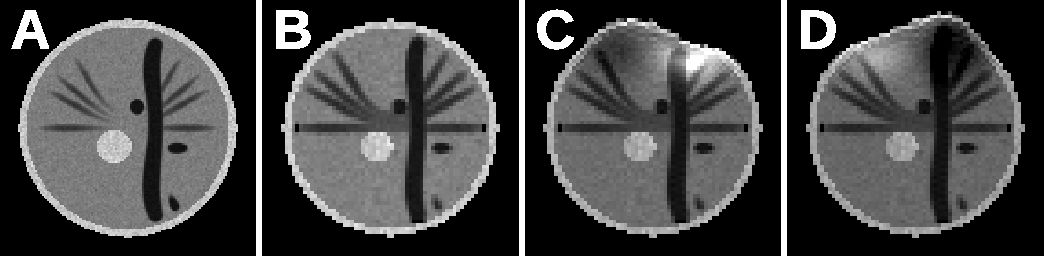
\includegraphics[width=0.95\columnwidth]{Fig01-Phantom}
   \caption{Ground-truth digital phantom.
   A) T2w; B) undistorted \textit{b0} volume;
   C, D) distorted \textit{b0} volumes with opposed phase 
   encoding directions, maximum displacement of 3.80~mm.}
   \label{fig:phantom}
\end{figure}

\subsection{Correction methods}
\label{sec:correction}
Three out of four methods presented in \autoref{sec:intro} were tested on the
  evaluation framework.
\Gls*{fmb} correction is the same as the one used for generating the distortion,
  working on the opposite direction.
Normally distributed noise was added to the synthetic field map (\gls*{snr}=20dB)
  before correction, for a more realistic evaluation.
\Gls*{reb} correction is implemented in \emph{FSL} (\texttt{topup}), and it demands for the \textit{b0}
  of the reverse-encoding simulation.
In this second case, the \gls*{vsm} is inferred from the differences between the two corresponding 
  \textit{b0}.
Finally, we included \Gls*{t2b} methods with \emph{ANTs} (\url{stnava.github.io/ANTs}),
  fine-tuned for \textit{b0}-to-T2w registration.
To this end, we used a multi-resolution scheme with 3 levels of subsampling and smoothing,
  mutual information metric, and the symmetric diffeomorphic transform model.
Several configurations of kernel widths for the regularization smoothers were tested, and finally
  selected 0.5/1.0 voxels (gradient/deformation fields, respectively) for its best result.
Additionally, undistorted images are corrected for dropout using the determinant of the Jacobian 
  of the deformation field.

\subsection{Evaluation}
\label{sec:evaluation}
The original phantom, one distorted version, and the corrected instances are then connected to a
  \gls*{dwi} reconstruction and tractography pipeline.
Additionally, the original tissue probability maps are also distorted and corrected to provide
  tractography with the required \gls*{wm} masks.
These maps are also used in a final assessment module.

The framework supports two different methods for \gls*{dwi} reconstruction and deterministic
  tractography:
1) \emph{Diffusion Toolkit} (\url{trackvis.org/dtk}) %\cite{wang_diffusion_2007}
  for \gls*{dti}, is configured with 10 random seeds per voxel by default; and
2) \emph{MRTrix} %\cite{tournier_mrtrix:_2012}
  (\url{www.brain.org.au/software/mrtrix}) for \gls*{hardi}, with default parameters
  set to use constrained spherical deconvolution, maximum harmonic order of 6, and
  150000 desired tracks.
For both options, the seeding regions can be set to use either the distorted-corrected 
  \gls*{wm} mask, or the regions used to generate the ground-truth.
This second seeding strategy mimics the usual procedure on real data,
  where regions are typically mapped from the anatomically correct T1w.

The evaluation framework is completed by automated assessment modules.
We evaluated three characteristics of the correction methods.
Firstly, we assessed the geometrical correctness reporting overlap indices of three tissue
  probability maps (namely \gls*{csf}, \gls*{wm}, and \gls*{gm}), weighting the average by
  tissue volumes.
Secondly, to evaluate the quality of the actual signal dropout correction, we studied the 
  similarity volume by volume computing the $\ell_1$-norm correlation index.
We report this score on the \textit{b0} and the average of the remaining \gls*{dwi} volumes.
Thirdly, we studied the impact on the connectivity matrices reporting the number of 
  false positives (nonexistent connections in the gold-standard) and false negatives 
  (or missed connections).
\section{RESULTS AND DISCUSSION}
\label{sec:results}
The results of the proposed experiments are summarized
in \autoref{fig:results} and \autoref{table:results}.
The remaining of this section provides extended descriptions
and interpretation of results.


\begin{table}[!t]
\caption{Accuracy results}
\label{table:results}
\begin{center}
\begin{tabular}{c||cccc|cc}
\hline
 & \multicolumn{4}{c|}{ Overlap (Jaccard Index, \%)} & \multicolumn{2}{c}{ Signal Correlation (\%)} \\
\hline
 & Av. & \gls*{csf} & \gls*{wm} & \gls*{gm} & \textit{b0} & \glspl*{dwi} \\
\hline
\gls*{fmb} & $93.00$ & $88.57$ & $96.74$ & $94.02$ & $80.05$ & $96.26\pm.06$ \\
\hline
\gls*{reb} & $96.64$ & $94.31$ & $98.26$ & $96.75$ & $91.00$ & $97.65\pm.03$ \\
\hline
\gls*{t2b} & $79.19$ & $66.31$ & $89.85$ & $82.14$ & $64.58$ & $90.10\pm.13$ \\
\hline
\end{tabular}
\end{center}
\end{table}

\begin{figure*}[tpb]
   \centering
   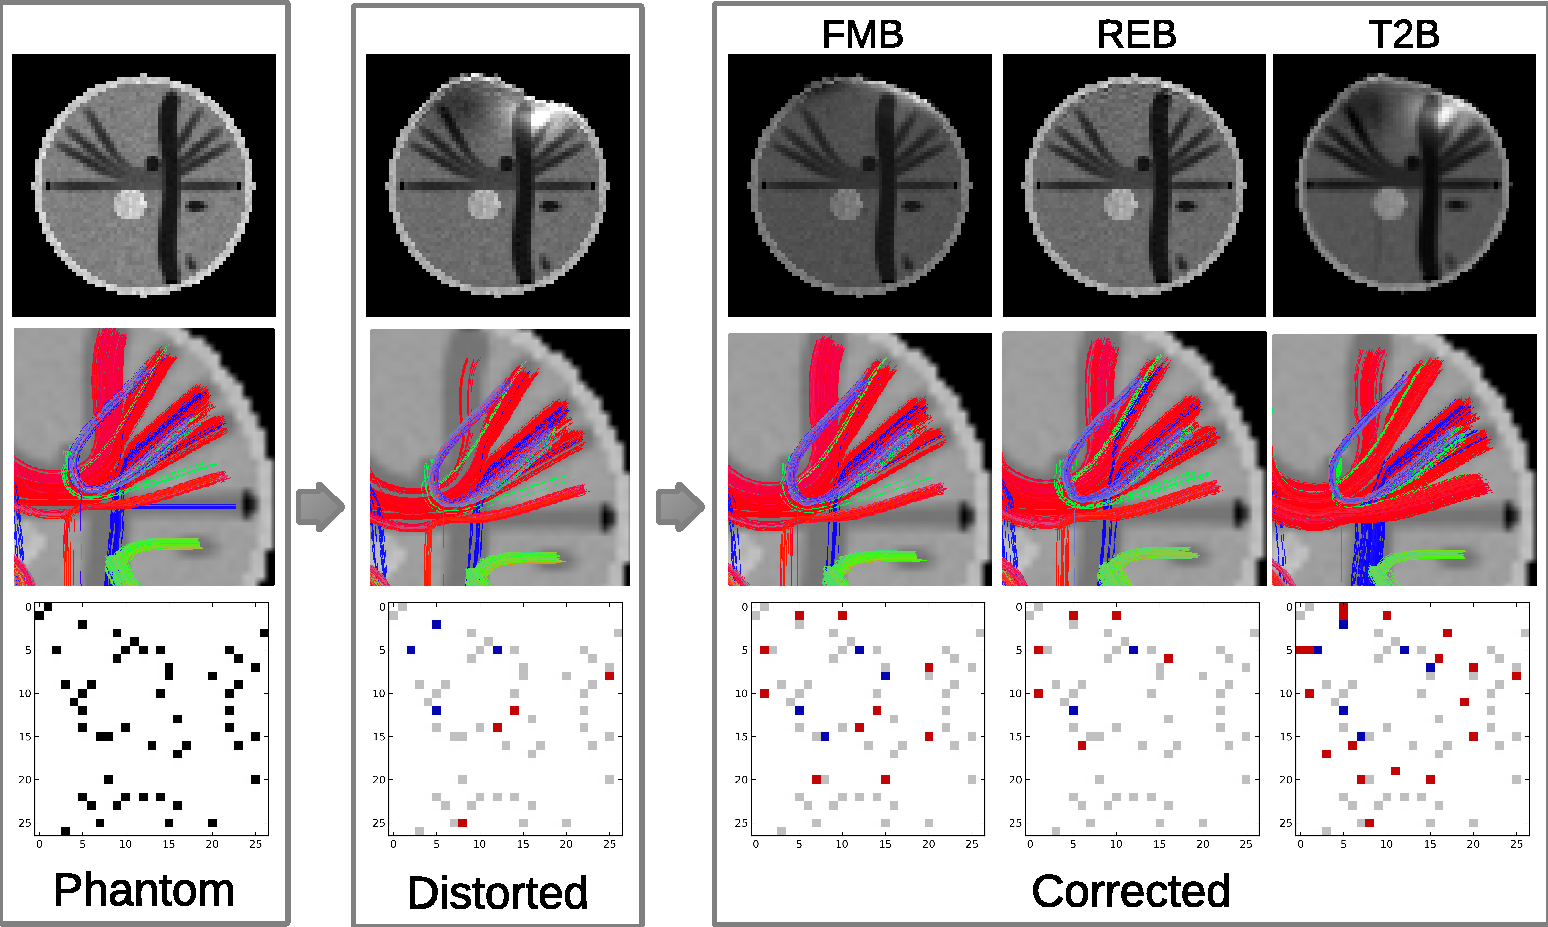
\includegraphics[width=0.9\textwidth]{Fig02-Results}
   \caption{The three major stages of the evaluation framework,
   along with the associated visual results. First row represents
   a coronal section of the \textit{b0} volume. In second row, the outcome
   of tractography, showing only tracks that connect two different
   network nodes. Third row shows the associated connectivity matrix. }
   \label{fig:results}
\end{figure*}


\subsection{Geometrical correctness}

The three methods under study achieved good results in
terms of geometrical accuracy, as it is shown in the first
row of \autoref{fig:results}. The best numerical scores
were obtained with the \gls*{reb} method (\autoref{table:results}),
that achieved a weighted average overlap of $96.64\%$. Second
best were obtained with \gls*{fmb}. Geometrical correctness
is fundamental in connectivity analysis to spatially locate the
\glspl*{roi} that will define the nodes of the final connectivity
matrix. The clear difference of accuracy between \gls*{reb} and \gls*{fmb}
with respect to \gls*{t2b} infers the latter may not be
an appropriate method for susceptibility correction.

\subsection{Signal loss recovery}

A second workflow evaluated the different correction 
methodologies to show the similarity of the recovered
signal with respect to the original (undistorted).
In this second study, \gls*{reb} performed significantly
better than the other two methods, as reported
in \autoref{table:results}. \gls*{reb} scored a $91.0\%$
similarity index for the \textit{b0} volume and an average $97.65\%$
for the remaining 31 \glspl*{dwi}. Again, the second
qualified was \gls*{fmb}, which achieved very close results
for the \glspl*{dwi} ($96.26\%$) but not as good for the \textit{b0}
volume. Visual inspection of the recovered data confirm the 
results presented in the Table (\autoref{fig:results}, first
row). Finally, \gls*{t2b} confirmed that its correction
can not be compared, even when using the intensity compensation
based on the determinant of the deformation field.

\subsection{Impact on tractography and connectivity}

The gold-standard contained a total of 1800 valid tracks
connecting regions, with an average length of $40.88\pm8.06$mm.
The corresponding connectivity matrix presented 25 connections 
between the total of 27 different seeding regions.

The distortion of the phantom caused 2 false positives (inexistent 
connections created by distortion) and 2 false negatives 
(connections vanished). The correction methods had an adverse impact
on connectivity. Only \gls*{reb} could recover one lost connection
but increasing the false connections count to 3.
\gls*{fmb} ranked second, with 5 false and 2 lost connections.
Finally, \gls*{t2b} presented 9 false and 3 lost connections.

For the shake of completeness, we also document the outcome
of tractography after each correction method. After distortion,
we obtained 1750 tracks and a characteristic length of 
$40.64\pm8.12$mm.
\gls*{fmb} produced 1900 tracks/$40.53\pm8.07$mm., \gls*{reb}
obtained 2200 tracks/$41.15\pm7.60$mm., and 2500 
tracks/$40.60\pm7.81$mm. for \gls*{t2b}. Although track counting has
been used as a measurement of success and as a weight of connectivity 
strength, the number of tracks produced by tractography strongly rely
on the seeding performed and the smoothing caused by interpolations 
within correction methodologies.

\subsection{Discussion}

Even though all the surveyed methods produced visually 
sound results, our study suggested that \gls*{reb} is the 
most accurate methodology for correction of susceptibility-induced
distortions in \gls*{dwi}. Moreover, \gls*{reb} also achieved
the best results in terms of connectivity, being able to recover
one of two lost connections after distortion. \Gls*{fmb} achieved 
very positive scores. Finally, the \gls*{t2b} method did not achieve
the necessary high-standards to recommend its use. We understand
that specific methods with anisotropic regularization that completely
restrict deformations to the phase-encoding axis would perform
significantly better as compares to the standard methods in this study.

One relevant limitation of this work is that the \gls*{fmb} is
used both in distortion creation and correction, what could
bias results. Nonetheless, \gls*{reb} performed better that \gls*{fmb}.
A second limitation is found on the impossibility of integrating the
point spread function-based methods for two reasons.
First, the unmet need of a point spread function map consistent
with the synthetic phase-difference map. Second, to our knowledge,
there are no implementations of the method readily available.
In practice, this second limitation is narrowed down by the
fact that typical acquisition protocols usually include one or more
datasets among field mapping, reversed-encoding \textit{b0} or T2,
but they do not include the point-spread function mapping.
\section{CONCLUSION}

This paper proposes an evaluation framework to
comprehensively analyze the impact of susceptibility
induced distortion on tractography from \gls*{dmri}
data. Inaccuracy on tractography produce errors
and increased variability in subsequent connectivity 
analyses of the whole-brain. Specially, in regions 
influenced by  significant distortion.
We publicly release the framework and also contribute
with the evaluation of the most widely-used and
readily-available correction methodologies. 
This work shows that \gls*{dmri} should be corrected
for susceptibility-induced artifacts prior to tractography
and connectivity analyses. In that sense, the \gls*{reb} 
method was the best classified
in two of the three rankings (geometric 
correctness and signal recovery), whereas \gls*{fmb}
achieved the lowest impact on the connectivity matrix
extracted from tractography.


\addtolength{\textheight}{-12cm}   % This command serves to balance the column lengths
                                  % on the last page of the document manually. It shortens
                                  % the textheight of the last page by a suitable amount.
                                  % This command does not take effect until the next page
                                  % so it should come on the page before the last. Make
                                  % sure that you do not shorten the textheight too much.

%%%%%%%%%%%%%%%%%%%%%%%%%%%%%%%%%%%%%%%%%%%%%%%%%%%%%%%%%%%%%%%%%%%%%%%%%%%%%%%%



%%%%%%%%%%%%%%%%%%%%%%%%%%%%%%%%%%%%%%%%%%%%%%%%%%%%%%%%%%%%%%%%%%%%%%%%%%%%%%%%



%%%%%%%%%%%%%%%%%%%%%%%%%%%%%%%%%%%%%%%%%%%%%%%%%%%%%%%%%%%%%%%%%%%%%%%%%%%%%%%%
%\section*{APPENDIX}
%
%Appendixes should appear before the acknowledgment.
%
%\section*{ACKNOWLEDGMENT}
%
%The preferred spelling of the word �acknowledgment� in America is without an �e� after the �g�. Avoid the stilted expression, �One of us (R. B. G.) thanks . . .�  Instead, try �R. B. G. thanks�. Put sponsor acknowledgments in the unnumbered footnote on the first page.



%%%%%%%%%%%%%%%%%%%%%%%%%%%%%%%%%%%%%%%%%%%%%%%%%%%%%%%%%%%%%%%%%%%%%%%%%%%%%%%%

\bibliographystyle{IEEEtran}
% argument is your BibTeX string definitions and bibliography database(s)
\bibliography{IEEEabrv,99-references}



\end{document}
